\documentclass[10pt]{article}
\usepackage[top=1in, bottom=1in, left=1in, right=1in]{geometry}
\usepackage{float}
\usepackage{color}
\usepackage{listings}
\usepackage{picture}
\usepackage{hyperref}
\usepackage{graphicx}
\usepackage[utf8]{inputenc}

% Used for the figures that have been inserted into the document.
\floatstyle{plain} 
\restylefloat{figure}

% Used so as not to indent paragraphs.
\setlength\parindent{0pt}

% Used for commenting purposes.
\definecolor{my-gray}{gray}{0.45}

\begin{document}

\title{\textbf{\textsc{Assignment 1}}}
\author{MA226 : Monte Carlo Simulation \\
			Rohit Rangan \\
			Roll No : 11012333 \\
			IIT Guwahati}
\date{}
\maketitle

\begin{center}
	\line(1, 0){15cm}
\end{center}

\section{Question}
The Newton-Raphson method is an iterative process for solving the root of the equation $f(x) = 0$. According to the method, starting with an initial guess of $x_{0}$, we apply the iterative formula $$x_{n+1} = x_{n} - \frac{ f(x_{n})}{f^{'}(x_{n})}$$ where $f^{'}(x)$ denotes the derivative of the function. The iteration stops until we arrive at an acceptable limit $\left|x_{n+1} - x_{n}\right| < \epsilon$, where $\epsilon$ is some pre-specified tolerance value. \medskip

Write a program to approximate the root of the equation $$3x^2 - e^x = 0,$$ to within a tolerance of $10^{-5}$. Give the steps in your code and the result of executing your code. Give an explanation as to why your answer is reasonable.



From the graph, it is very clear that there are three solutions to the equation, the first one lies in the interval $[-1,0]$, the second one lies in the interval $[0,1]$ and the third one lies in the interval $[3,4]$. \medskip

\subsection{R Code for Calculating the Roots}

\lstinputlisting[language=R, tabsize=4, keywordstyle=\color{blue}, commentstyle=\color{my-gray}]{Ass1R.R}

\medskip

\subsection{Solution and its Interpretation}

After executing the \verb+find_root+ method declared above in \verb+R+, the equation $$3x^2 - e^x = 0$$ has the solutions:-  $$-0.4589623,  0.9100076\: and\: 3.7330790$$ \medskip

If we put the values back into the equation, we have:- 

\begin{eqnarray}
	f(-0.4589623) &=& 1.099106 \times 10^{-7} \\
	f(0.91000760) &=& 8.186546 \times 10^{-8} \\
	f(3.37330790) &=& 5.557389 \times 10^{-7}
\end{eqnarray}

From these values, we can see that the solutions are accurate to the order of $10^{-7}$. Hence $ \epsilon = 10^{-5}$ we had chosen initially provides good, but approximate solutions to the given equation.
\section{Solution in R}
\begin{figure}[H]
	\centering
	\resizebox{0.5\textwidth}{!}{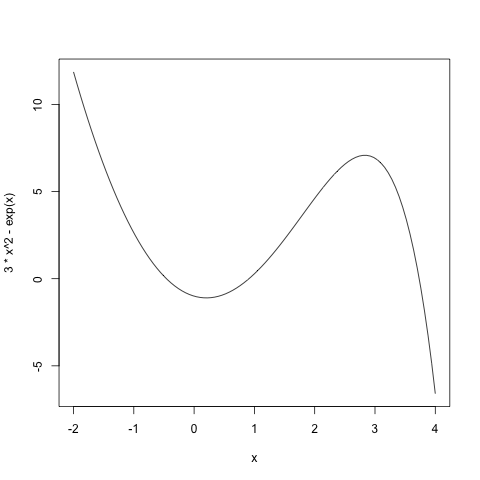
\includegraphics{Plot.png}}
	\caption{Graph of $3x^2 - e^x$ in the interval $[-2,4]$}
\end{figure}
\section{Solution in C++}
 \begin{figure}[H]
	\centering
	\resizebox{0.5\textwidth}{!}{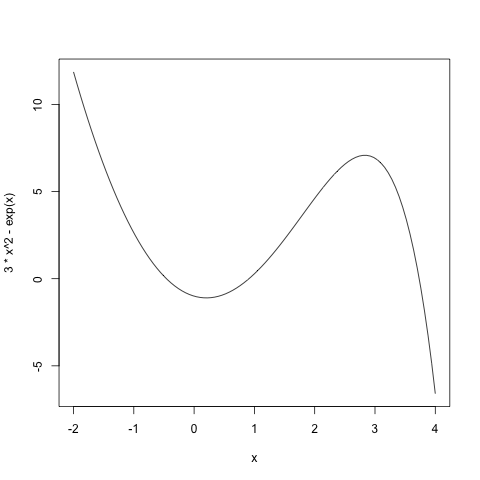
\includegraphics{Plot.png}}
	\caption{Graph of $3x^2 - e^x$ in the interval $[-2,4]$}
\end{figure}

\subsection{C++ Code for Calculating the Roots}
\lstinputlisting[language=C++, tabsize=4, keywordstyle=\color{blue}, commentstyle=\color{my-gray}]{Ass1c++.cpp}

\subsection{Solution and its Interpretation}

After executing the program, the equation $$3x^2 - e^x = 0$$ has the solutions:-  $$-0.458962,  0.910008\: and\: 3.73308$$ \medskip

If we put the values back into the equation, we have:- 

\begin{eqnarray}
	f(-0.458962) &=& -9.058031 \times 10^{-7} \\
	f(0.910008) &=& 1.272147 \times 10^{-6} \\
	f(3.373308) &=& -1.885344 \times 10^{-5}
\end{eqnarray}

From these values, we can see that the solutions are accurate to the order of $10^{-5}$. Hence $ \epsilon = 10^{-5}$ we had chosen initially provides good, but approximate solutions to the given equation.
\section{Conclusion}

We have solved the equation $3x^2 - e^x = 0$, using the Newton-Raphson method. The solutions to the given equation have been obtained to an accuracy of $\pm 10^{-7}$ in \texttt{R} and $\pm 10^{-5}$ in \texttt{C++}.\medskip

The reason for the higher accuracy in \texttt{R} than compared to \texttt{C++} is because \texttt{R} can do higher precision floating point arithmetic than \texttt{C++}.

\end{document}
